\documentclass[11pt, titlepage]{article}
\usepackage{amsmath,amsthm,amssymb}
\usepackage{hyperref, pgf, tikz}
\usepackage{fancyhdr}
\usetikzlibrary{arrows}
\usepackage[margin=1.25in]{geometry}
\usepackage{graphicx}                     
\pagestyle{fancy}
\usepackage{array}
%\usepackage{wrapfig}

\lhead{Lab \#1}
\rhead{\thepage}
\cfoot{}

\title{Projectile Motion: The Ballistic Pendulum \\ \ \\ \large Lab \#2}
\author{Name: Avery Karlin \\ Partner: Alon Levin}
\date{}
\begin{document}

\maketitle

\begin{center}
\LARGE Projectile Motion: The Ballistic Penudulum
\end{center}

\section*{Objective}
The objective of the lab is to 
\section*{Introduction}
The main theory used within the lab is that of Newton's Second Law: $$F_{net} = ma,$$ such that within an Atwood machine, or two masses on opposite sides of a pulley, the force of gravity, $F_g = mg$, works in opposite directions. Since the pulley is all joined together, the total acceleration of the system is constant. In addition, due to the real world constraints, we must also subtract the force of friction (both from the pulley and from the surrounding air), and add the mass of the pulley to the total mass.

Thus, $F_{net} = (m_1 + m_2 + m_{pulley})a = m_1g - m_2g - f$, where f is the force of friction. This can then be rewritten as $$a = \frac{m_2 - m_1)g - f}{m_1 + m_2 + m_{pulley}}.$$ This can then be taken when a = 0, such that the frictional force of the system, divided by the gravitational constant to find the mass that must be subtracted out due to friction: $$a = \frac{(m_2 - m_1 - m_f)g}{m_1 + m_2 + m_{pulley}}.$$

The acceleration of the actual experimental system is done through determining the time the mass takes to fall a specific distance, such that the equation, $$y = v_0t + \frac{1}{2}at^2,$$ can be used to find the acceleration of the system, assuming it is constant. It can then be modified due to starting from rest, solving for acceleration to: $$a = \frac2y}{t^2}.$$
\section*{Procedures and Results}

First, the entire Atwood machine setup must be built, with equal masses on both sides, adding mass to one side until a = 0, such that the added mass is $m_f$, the mass needed to compensate for friction, then we added mass to the descending side, and measuring the amount of time it took to fall a specific distance. After, we tested using different masses on both, but preserving the relative mass, creating different frictional masses/forces on each, measuring the resultant acceleration.

Next, equal masses are put on both sides again, determining the frictional mass, then slowly moving several grams more each trial to the descending mass to change the force of the two sides, while keeping the total mass constant, taking all calculations by the same methods as during the first, measuring the resultant acceleration.

\begin{figure}[p]
\centering
\hspace*{-10.5cm}
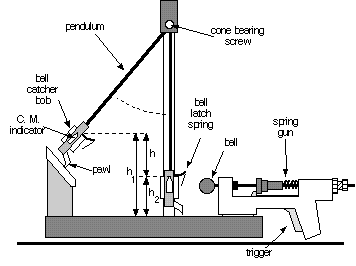
\includegraphics[scale=0.15, angle=270]{lab2.jpg}
\vspace*{19cm}
\end{figure}

\begin{center}
$$\text{Height of} h_2 \text{of pointer with pendulum catch in closest-to-average notch number} = $$
$$\text{Height of} h_1 \text{of pointer with pendulum freely suspended} = $$
$$h = h_2 - h_1 = $$
$$\text{Mass of ball m} = $$
$$\text{Mass of pendulum M (bob and support)} = $$
\begin{tabular}
{|m{7em}|m{7em}|}
\hline
Trials & Notch Number of Pendulum Catch \\
\hline
1 & \\
\hline
2 & \\
\hline
3 & \\
\hline
4 & \\
\hline
5 & \\\
\hline
Average & \\
\hline
\end{tabular}

$$\text{Vertical distance of fall, y} = $$
$$v_{x_o} \text{(calculated)} = $$
$$\text{Percent difference between results of part A and B} = $$
\begin{tabular}
{|m{7em}|m{7em}|}
\hline
Trials & Range\\
\hline
1 & \\
\hline
2 & \\
\hline
3 & \\
\hline
4 & \\
\hline
5 & \\\
\hline
Average & \\
\hline
\end{tabular}

\begin{tabular}
{|m{7em}|m{7em}|}
\hline
Angle of projection & Average range \\
\hline
$20^o$ & \\
\hline
$30^o$ & \\
\hline
$40^o$ & \\
\hline
$50^o$ & \\
\hline
$60^o$ & \\
\hline
$70^o$ & \\
\hline
\end{tabular}

\section*{Discussion}
Sample calculations for the non-measured data are as shown:

%Add more discussion here

\section*{Conclusion}


\end{document}
